The primary use scenario of \abbr{EWAS} is the detection of a missile-launch candidate that may threaten the Baltic region, followed by Ground Segment-directed tracking, impact-area assessment, and automatic dispatch of a preliminary warning to authorized national authorities. The preliminary warning is issued only after the two selected \abbr{LEO} satellites have returned tracking observations and the Ground Segment has produced a refined trajectory and impact-area estimate. Operator review follows the first warning; it does not gate its dispatch.

\textbf{Primary actors:} Ground Segment mission-control operators, the \abbr{GEO} detection layer, selected \abbr{LEO} tracking satellites, and external authorized national authorities.

\textbf{Event flow:}
\begin{enumerate}
    \item A \abbr{GEO} infrared sensor detects a candidate thermal event and performs preliminary onboard noise filtering and event characterization.
    \item The \abbr{GEO} satellite securely reports the event location, time and available confidence information to the Ground Segment.
    \item Ground Segment coordination and command-and-control functions assess the available constellation geometry, select two suitable \abbr{LEO} satellites close to the event with adequate visibility, and prepare tracking requests.
    \item The Ground Segment routes tracking commands through an available ground-station link or, where supported and available, via an inter-satellite relay path. Inter-satellite coordination may be used when needed. Availability and timing of these paths remain subject to verification.
    \item The two cued \abbr{LEO} satellites orient their sensors, collect complementary observations and compute a preliminary trajectory estimate using the available tracking data.
    \item Their encrypted observations and preliminary estimate are delivered to the Ground Segment. Ground Station Network services securely receive and forward the information to the Data Processing System.
    \item The Data Processing System performs multi-source fusion, calculates a refined trajectory estimate and an impact-area estimate with associated uncertainty, and evaluates the potential relevance to the Baltic region.
    \item Once the two-satellite assessment is available, the Ground Segment Early Warning System automatically generates and sends a clearly marked \emph{preliminary warning} to the interfaces of the relevant authorized national authorities. Sending is not conditional on operator confirmation. The mission-level requirement is delivery within 60 seconds of the first \abbr{GEO} detection; its feasibility must be demonstrated by an end-to-end latency analysis.
    \item The Mission Control Center presents the event and transmitted warning to the operator. Following review, authorized personnel can confirm the assessment, request an update, or cancel a warning using the established operational procedure. Any subsequent update is sent to the same appropriate authorities.
    \item The Ground Segment Data Archiving System stores the applicable raw and processed records, warning versions, acknowledgements, and audit logs, irrespective of the subsequent operator decision. Archived data are used only for the purposes allowed by R-004.
\end{enumerate}

No separate User and Data Segment is part of the system baseline. The authorities' receiving interfaces are external to \abbr{EWAS}; any subsequent public warning is their responsibility.

\begin{figure}[H]
    \centering
    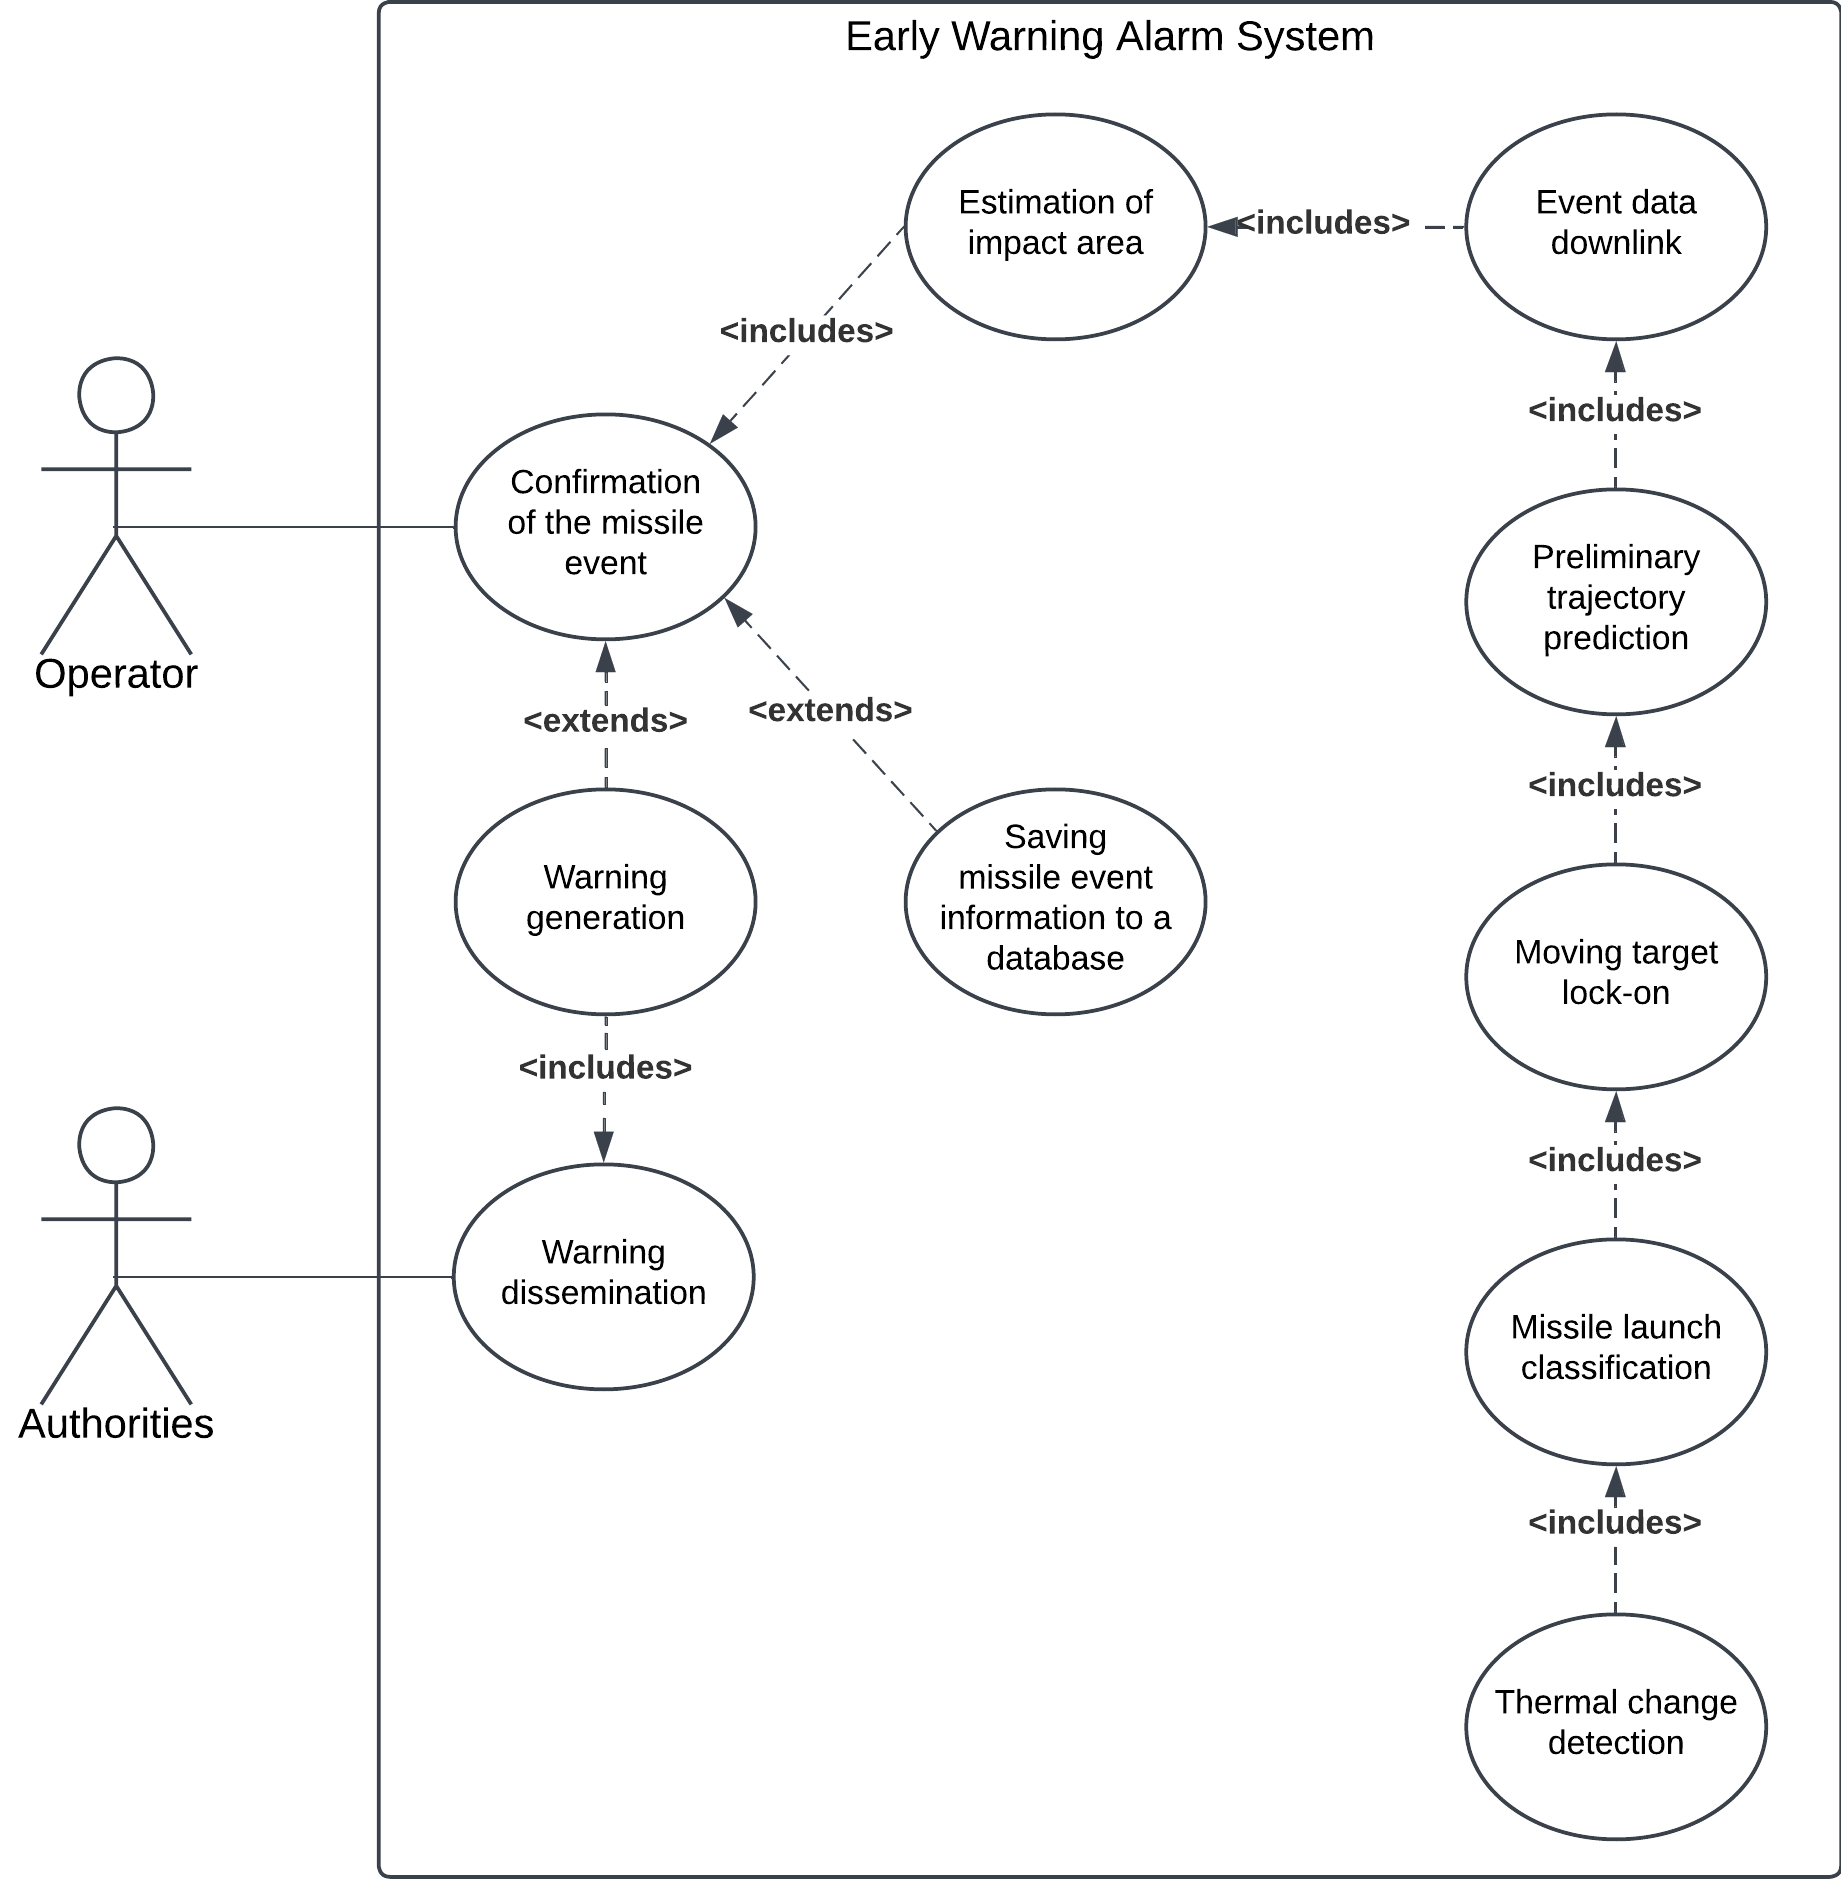
\includegraphics[width=0.96\textwidth]{Figures/use_scenario.png}
    \caption{Revised system operational sequence: ground-selected LEO tracking and warning after LEO observations}
    \label{fig:use_case_diagram}
\end{figure}
